\documentclass[border=5pt]{standalone}
\usepackage{tikz}
\usepackage{tikz-3dplot}
\usetikzlibrary{arrows.meta, 3d, perspective, calc}
\usepackage{amsmath}
\begin{document}
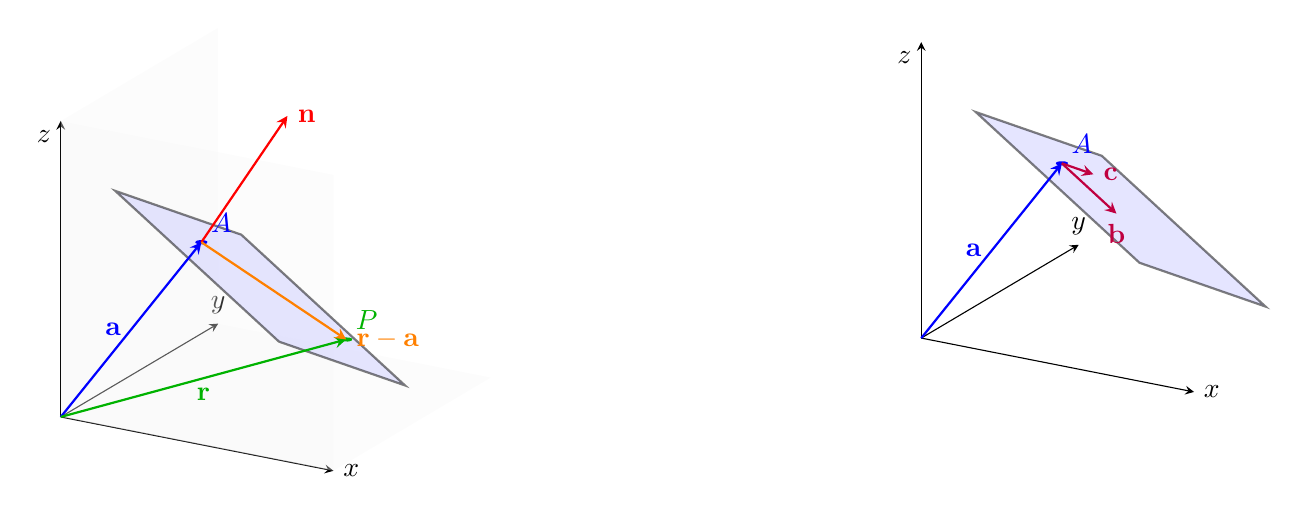
\begin{tikzpicture}[scale=0.8, >=stealth, 3d view={30}{20}]
    \begin{scope}[shift={(-5,-5,0)}]
    % Coordinate system with better perspective
    \draw[->] (0,0,0) -- (5,0,0) node[right]{$x$};
    \draw[->] (0,0,0) -- (0,5,0) node[above]{$y$};
    \draw[->] (0,0,0) -- (0,0,5) node[below left]{$z$};

    % Draw axes planes for better 3D perception (semi-transparent)
    \fill[gray!10,opacity=0.2] (0,0,0) -- (5,0,0) -- (5,5,0) -- (0,5,0) -- cycle;
    \fill[gray!10,opacity=0.2] (0,0,0) -- (5,0,0) -- (5,0,5) -- (0,0,5) -- cycle;
    \fill[gray!10,opacity=0.2] (0,0,0) -- (0,5,0) -- (0,5,5) -- (0,0,5) -- cycle;

    % Draw the plane
    \draw[thick, fill=blue!20, opacity=0.5]
        (1,0,4) -- (4,0,2) -- (4,4,0) -- (1,4,2) -- cycle;

    % Draw point A on the plane
    \coordinate (A) at (2,1,3);
    \fill[blue] (A) circle (0.1) node[above right] {$A$};

    % Draw position vector to A
    \draw[->,thick,blue] (0,0,0) -- (A) node[midway,left] {$\mathbf{a}$};

    % Draw normal vector from a point on the plane
    \draw[->,thick,red] (A) -- ($(A)+(1,1,2)$) node[right] {$\mathbf{n}$};

    % Draw another point P on the plane
    \coordinate (P) at (3.5,3,1);
    \fill[green!70!black] (P) circle (0.1) node[above right] {$P$};

    % Draw position vector to P
    \draw[->,thick,green!70!black] (0,0,0) -- (P) node[midway,below] {$\mathbf{r}$};

    % Draw r-a vector
    \draw[->,thick,orange] (A) -- (P) node[right] {$\mathbf{r} - \mathbf{a}$};

\end{scope}
\begin{scope}[shift={(5,5,0)}]
     % Coordinate system with better perspective
     \draw[->] (0,0,0) -- (5,0,0) node[right]{$x$};
     \draw[->] (0,0,0) -- (0,5,0) node[above]{$y$};
     \draw[->] (0,0,0) -- (0,0,5) node[below left]{$z$};

    % Draw the plane
    \draw[thick, fill=blue!20, opacity=0.5]
        (1,0,4) -- (4,0,2) -- (4,4,0) -- (1,4,2) -- cycle;

        % Draw point A on the plane
    \coordinate (A) at (2,1,3);
    \fill[blue] (A) circle (0.1) node[above right] {$A$};
    % Draw position vector to A
    \draw[->,thick,blue] (0,0,0) -- (A) node[midway,left] {$\mathbf{a}$};

    % Draw vectors in the plane
    \draw[->,thick,purple] (A) -- ($(A)+(1,0,-0.6666)$) node[below] {$\mathbf{b}$};
    \draw[->,thick,purple] (A) -- ($(A)+(0,1,-0.5)$) node[right] {$\mathbf{c}$};

\end{scope}
\end{tikzpicture}
\end{document}
